\section{Application Scenarios}
In order to respect the fairness, legitimacy and power of assets, we have made the design of the distribution model concise, clear and effective. Combined with the ecological characteristics of Nebulas, more incentives and economic game scenarios are handed over to application scenarios. With this principle, incentive and consumption scenarios within the application scenario can be more varied and diverse. In this chapter, we will explore some prospects for existing and future application scenarios in Nebulas. As shown in Figure \ref{fig:nax_ecosys}, we can clearly outline the positive incentives of NAX in the Nebulas ecosystem.

\begin{figure}[h]
  \centering
  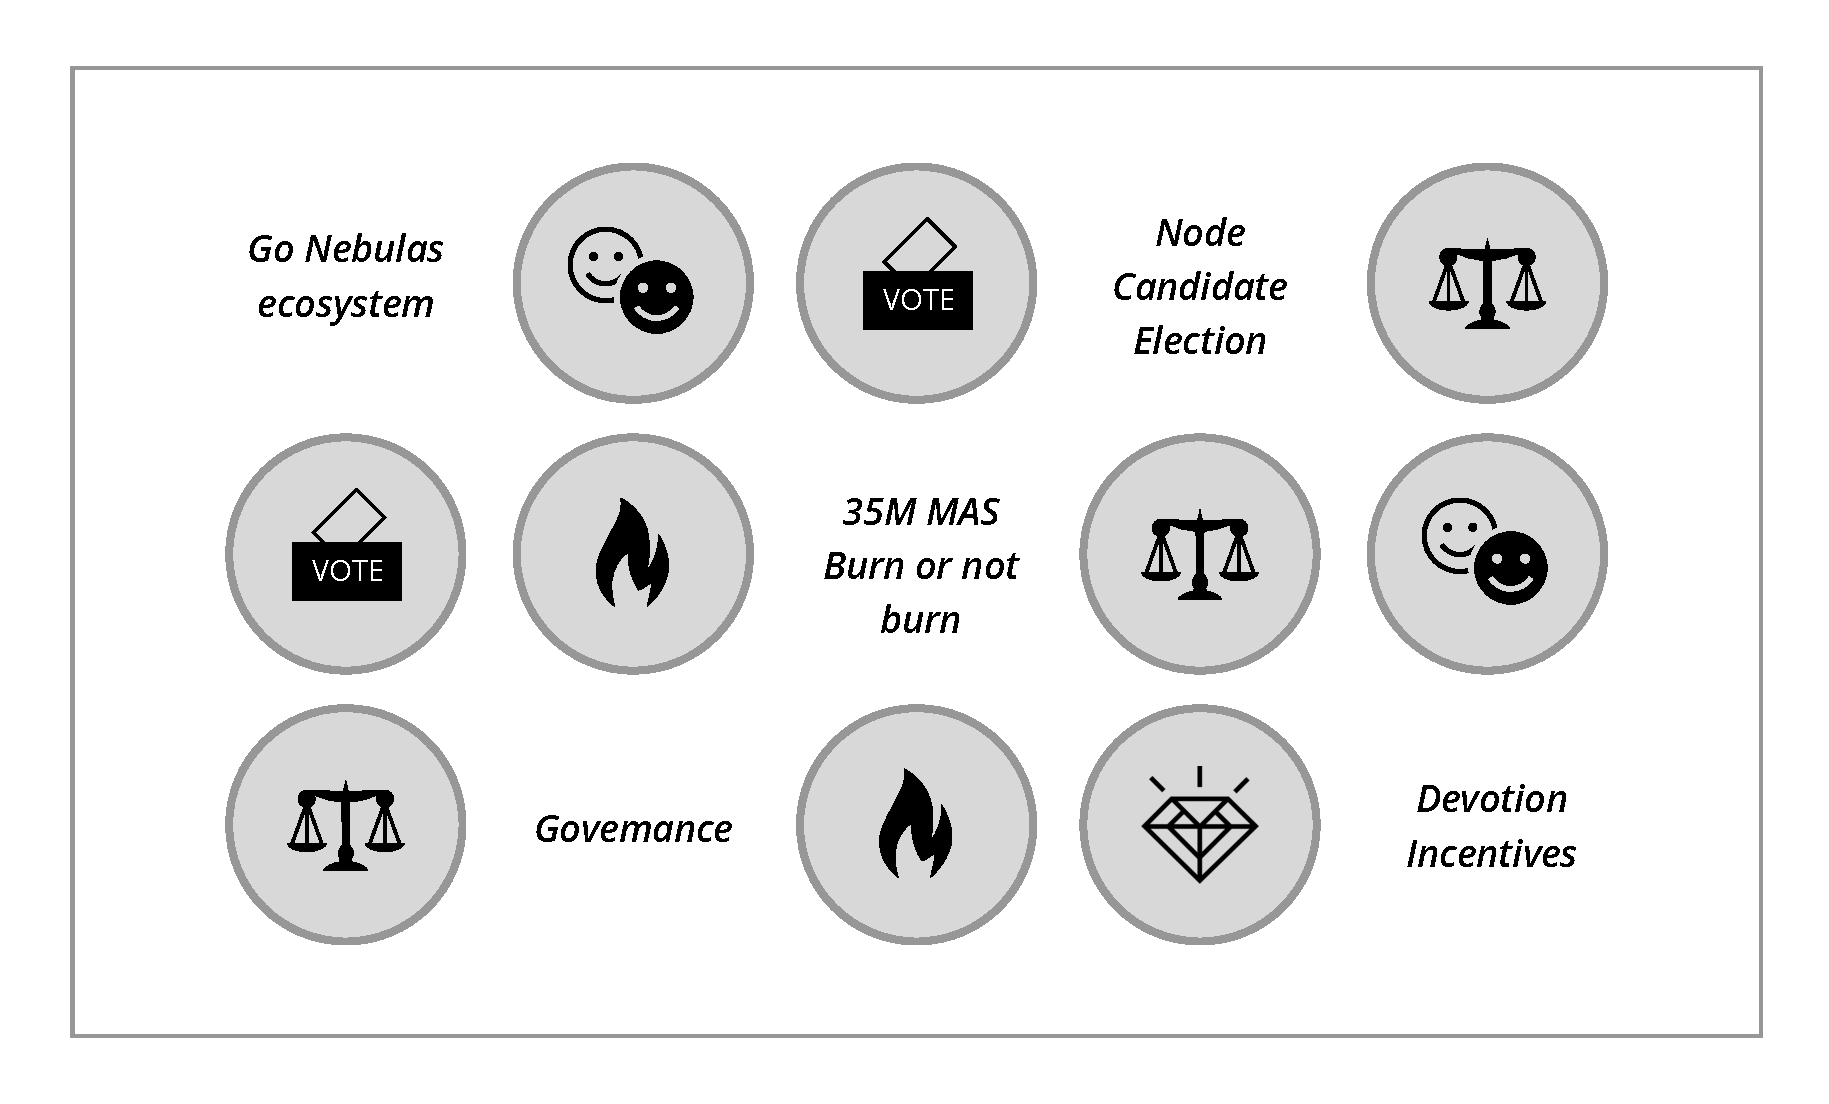
\includegraphics[width=0.6\textwidth]{../common/usecases.pdf}
  \caption{NAX usage scenarios in the nebula ecosystem\label{fig:nax_ecosys}}
\end{figure}

\subsection{Economic Contribution Incentive}
In the Nebulas white paper, the contribution-proof consensus algorithm Proof of Devotion (PoD) and the vision of Nebulas was shared: "Fair value for all via decentralized collaboration" and combined with the launch of the Go Nebulas platform in early 2019, Nebulas has constantly explored ecosystem contribution. These have all been important steps for Nebulas to move further towards the creation of the Autonomous Metanet. To this end, we put forward a unique pedge investment token as a proof of equity incentive which can be applied to different scenarios.

\subsubsection{Go Nebulas Incentive}
The Nebula Foundation will set aside no less than $3$ million in NAS to support projects on the Go Nebulas platform, and if needed, the Foundation will provide additional tokens. This tokens will be generated in staking and the resulting equity will be used to Incentivize the large and small contributions of users that are made on the Go Nebulas platform. For example, in addition to receiving NAS token as a reward, Go Nebulas contributors will also receive NAX incentives under the rules established by the Go Nebulas platform as an equity right contribution to the Nebulas ecosystem. The corresponding rights and governance can be exercised in the Nebulas ecosystem. Detailed incentives will be developed by Go Nebulas' operations team managers and community participants.

Incentives can be divided into the following categories:
\begin{enumerate}[\hspace{1cm}(a)]
	\item core infrastructure
	\item market expansion
	\item promotion
	\item creating proposals and participation
\end{enumerate}

In addition to being an important means of investing within community building and receiving NAX incentives, the Go Nebulas platform is an important use-case scenario for NAX. Utility scenarios include (but not limited to) the following categories:
\begin{enumerate}[\hspace{1cm}(a)]
	\item create and initiating a proposal
	\item passing and rejecting proposals
	\item staking twords the progress of the project
\end{enumerate}

\subsubsection{Foundation Core Member Incentive}
Members of the Nebulas Foundation core team which includes part-time and full-time staff will receive NAX benefits from the Foundation's staking as additional contribution which is in addition to receiving their appropriate salary.

\subsection{PoD Consensus Exploration}
With the advancement of Nebulas and the development of PoD, decentralization is the only way for Nebulas chain. NAX will play an important role in PoD by effectively combining PoD technology being developed to become the basis and direction of the new consensus algorithm. The previous section discussed the incentive scenarios for NAX in the ecosystem, and with the NAX single staking distribution method, the ways to obtained NAX include:

\begin{enumerate}[\hspace{1cm}(i)]
  \item contributing to the liquidity of assets
  \item investing in the continued construction of Nebulas
  \item participate in community governance
\end{enumerate}

From another perspective, it is not difficult to conclude that NAX can be seen as a contribution to the Nebulas ecosystem. As the name suggests, PoD is a proof of devotion and contribution. PoS (Proof of Stake) is the essence of the Nebulas blockchain which is more in line with blockchain collaboration. With different roles in ecosystem contribution as the basis for the block reward, we must not solely rely on the amount of processing power a entity controls such as PoW (Proof of Work).

When choosing a consensus committee members, users will be able to introduce the equity of NAX to influence the probability of the block generation. The election of consensus committee memebers, either through on-chain or off-chain method. Now let's take the off-chain node election as an example to explain the possible ways of describing the case. The final form will be based on the to-be published PoD technical documentation:

\begin{enumerate}[\hspace{1cm}(a)]
  \item node committee members are voted for via NAX
  \item members must burn a specified amount of NAX as well as pledging NAS
  \item nodes will be divided into multiple segments to enrich diversity
  \item the main network PoD consensus algorithm will introduce NAX as a parameter to influence the distribution of block equity
\end{enumerate}

\subsection{On-chain Governance Scenario}
Within the Nebulas ecosystem, there will be a variety of community selection and election activities. In order to increase participation in the community ecosystem, each activity will use NAX as a proof of equity and will be needed to play an important role in voting and incentive strategies.

For example a vote that will soon be proposed on how to handle the 35 million NAS community reserve tokens. The Nebulas Foundation has proposed to burn this tokens and we will ask the community to contribute options on the destruction (partially or fully). One possible solution is to launch a vote using NAX every month to burn the community's total reserved NAS \(\lambda\) \% , \(\lambda\) \% It is the current share of NAS staking rate in total circulation. We also encourage communities to provide more effective and proactive solutions to jointly determine the use of this part of assets.


\subsection{Ecosystem Advancement}
Developed by the Nebulas Foundation, the ecosystem products are an important element for the ecosystem use of the Nebulas blockchain. These products include the current and future Nebulas products incubated by the Foundation, such as NAS nano Pro ~\cite{NASnano}, Web Explorer ~\ Cite{explorer} and the Nebulas DEX. As NextDAO advances and community governance progresses, there will be many more NRC20 tokens and governance projects within the community. These new assets have a strong demand these ecosystem tools. With limited resources, we will require NRC20 project owner to contribute tokens in NAX to the platform. These tokens can also be used for activities and incentives for ecosystem projects. Token is used for the construction of the platform.
